\section{AST: Audio Spectrogram Transformer} \label{appendix:ast-paper}

\subsection{Overview}

\par Gong \textit{et al} in their 2021 paper titled \textit{AST: Audio Spectrogram Transformer} \cite{ast} proposed a model  which is convolution-free, solely attention-based that can capture long-range global context even in the lowest layers and is directly applied to an audio spectrogram. They also suggest a method for transferring knowledge from the ImageNet-pretrained Vision Transformer (ViT) to AST, which can greatly enhance performance.\par

\subsection{Datasets}
\begin{itemize}
\item AudioSet
\item ESC-50 
\item Speech Commands
\end{itemize}

\begin{figure}[h]
	\centering
	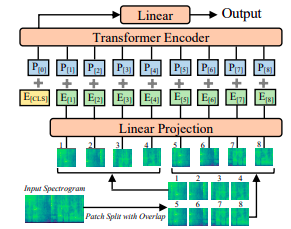
\includegraphics[width=0.5\linewidth]{assets/img/ast_methodology.png}
	\caption{Audio Spectrogram Transformer by Gong
	\textit{et al} (Courtesy \cite{ast})}
\end{figure}

\subsection{Methodology}
\begin{itemize}
\item A sequence of 128-dimensional log Mel filterbank (fbank) features is computed with a 25ms Hamming window every 10ms from the input audio waveform of t seconds. As a result, the AST receives a 128x100t spectrogram as input.
\item The spectrogram is then split into a sequence of N 16x16 patches with a time and frequency overlap of 6, where N is the number of patches and the Transformer's effective input sequence length.
\item Each 16×16 patch is then flattened into a 1 Dimensional patch embedding of size 768 using a linear projection layer. This layer is called patch embedding layer.
\item As the Transformer architecture does not capture the ordering of input tokens and the patch sequence added is also not in temporal order, so trainable positional embedding (also of size 768) is added to each of patch embedding which allows the model to capture the spatial structure of the 2D audio spectrogram. 
\item The CLS token is then appended to the beginning of the sequence, which is subsequently fed into the Transformer.
\item A Transformer model consists of many encoder and decoder layers. For classification tasks, AST only uses the encoder of the Transformer.
\item The [CLS] token output from the Transformer encoder serves as the audio spectrogram representation. The audio spectrogram representation is mapped to labels for classification using a linear layer with sigmoid activation.
\item AST model also allows cross-modality transfer learning as audio spectrograms format is very similar to images. So ImageNet-pretrained CNN weights are used as initial CNN weights for audio classification training. 
\end{itemize}

\subsection{Training procedure}
\begin{itemize}
\item Model is pre-trained using the ImageNet dataset. 
\item Model is trained  with a batch size of 12, uses binary cross-entropy loss and Adam optimizer.
\item The initial learning rate of 5e-5  is used for balanced set experiments and the model is trained for 25 epochs, the learning rate is then cut into half every 5 epochs after the 10th epoch.  
\item For full set experiments, the  initial learning rate of 1e-5 is used and the model is trained for 5 epochs, the learning rate is cut into half every epoch after the 2nd epoch.
\end{itemize}

\subsection{Conclusion}
\par Gong et al present Audio Spectrogram Transformer which is a convolution-free, purely attention-based model for audio classification which features a very simple architecture that gives superior performance.

